%%%%%%%%%%%%%%%%%%%%%%%%%%%%%%%%%%%%%%%%%%%%%%%%%%%%%%%%%%%%%%%%%%%%%%%%%%%%%%%%
% Preámbulo                                                                    %
%%%%%%%%%%%%%%%%%%%%%%%%%%%%%%%%%%%%%%%%%%%%%%%%%%%%%%%%%%%%%%%%%%%%%%%%%%%%%%%%

\documentclass[11pt,a4paper,titlepage,oneside]{report}

%%% RELACIÓN DE VARIABLES A PERSONALIZAR %%%
\def\lingua{gal}
%\def\lingua{esp} % descomenta esta liña se redactarás a memoria en español
%\def\lingua{eng} % descomenta esta liña se redactarás a memoria en inglés
\def\nome{Pablo Rodríguez Pérez}                             % substitúe aquí o teu nome
\def\nomedirectorA{Pablo Alejandro Calviño Padín}              % substitúe aquí o nome de quen dirixe
\def\nomedirectorB{Agustín Ricardo Rodríguez Fariña}             % duplica esta liña máis veces se o precisas, cambiando
                                                     % a letra final (A, B, C, D...): úsanse na portada.tex
\def\titulo{Desenvolvemento dunha Plataforma Web para a xestión Integral de Configuracións Técnicas no Entorno Universitario} % substitúe aquí o título do teu TFG
%\def\titulacion{gced}                               % descomenta esta liña e comenta a seguinte se es estudante do GCED
\def\titulacion{gei}
%\def\mencion{COMPUTACIÓN}                           % descomenta a mención que che corresponda se es estudante do GEI
%\def\mencion{ENXEÑARÍA DO SOFTWARE}
%\def\mencion{ENXEÑARÍA DE COMPUTADORES}
%\def\mencion{SISTEMAS DE INFORMACIÓN}
\def\mencion{TECNOLOXÍAS DA INFORMACIÓN}

%\def\renomearcadros{si} % descomenta esta liña se redactas a memoria en español e prefires que
                         % os "cuadros" e o "índice de cuadros" se renomeen
                         % a "tablas" e "índice de tablas" respectivamente

\usepackage{estilo_tfg}

% Lista de paquetes potencialmente interesantes (uso baixo demanda)

% \usepackage{alltt}       % proporciona o entorno alltt, semellante a verbatim pero que respecta comandos
% \usepackage{enumitem}    % permite personalizar os entornos de lista
% \usepackage{eurofont}    % proporciona o comando \euro
 \usepackage{float}       % permite máis opcións para controlar obxectos flotantes (táboas, figuras)
% \usepackage{hhline}      % permite personalizar as liñas horizontais en arrays e táboas
 \usepackage{longtable}   % permite construir táboas que ocupan máis dunha páxina
% \usepackage{lscape}      % permite colocar partes do documento en orientación apaisada
% \usepackage{moreverb}    % permite personalizar o entorno verbatim
% \usepackage{multirow}    % permite crear celdas que ocupan varias filas da mesma táboa
% \usepackage{pdfpages}    % permite insertar ficheiros en PDF no documento
% \usepackage{rotating}    % permite diferentes tipos de rotacións para figuras e táboas
% \usepackage{subcaption}  % permite a inclusión de varias subfiguras nunha figura
% \usepackage{tabu}        % permite táboas flexibles
% \usepackage{tabularx}    % permite táboas con columnas de anchura determinada

\usepackage[nounderscore]{syntax}
\usepackage{xfrac}
\usepackage{amsmath}
\usepackage[pdf]{graphviz}
\usepackage{tikz}
\usepackage{tikz-qtree}
\usepackage{pgf-umlcd}
\usepackage{pgf-umlsd}
\usepgflibrary{arrows}

%%%%%%%%%%%%%%%%%%%%%%%%%%%%%%%%%%%%%%%%%%%%%%%%%%%%%%%%%%%%%%%%%%%%%%%%%%%%%%%%
% Corpo                                                                        %
%%%%%%%%%%%%%%%%%%%%%%%%%%%%%%%%%%%%%%%%%%%%%%%%%%%%%%%%%%%%%%%%%%%%%%%%%%%%%%%%

\begin{document}

 %%%%%%%%%%%%%%%%%%%%%%%%%%%%%%%%%%%%%%%%
 % Preliminares do documento            %
 %%%%%%%%%%%%%%%%%%%%%%%%%%%%%%%%%%%%%%%%

 \begin{titlepage}
  
  \hspace*{128pt}
  \textcolor{udcpink}{{\fontencoding{T1}\fontfamily{phv}\selectfont Facultade de Informática}}\\[-32pt]

  \begin{center}
    
\includegraphics[scale=0.3]{imaxes/udc}\\[25pt]

    {\large TRABALLO FIN DE GRAO \\
            \nometitulacion \\
            \nomemencion } \\[10pt]

    \carimbo \\[25pt]

    \begin{huge}
      \begin{spacing}{1.3}
        \bfseries \titulo
      \end{spacing}
    \end{huge}
  \end{center}
  
  \vfill
  
  \begin{flushright}
    {\large
    \begin{tabular}{ll}
      {\bf Estudante:} & \nome \\
      {\bf Dirección:} & \nomedirectorA \\
                       & \nomedirectorB \\ % duplica esta liña máis veces se o precisas, cambiando
                                           % a letra final (A, B, C, D...); define eses nomes no memoria_tfg.tex
    \end{tabular}}
  \end{flushright}
  \rightline{A Coruña, \datasimple.}
\end{titlepage}

 %\dedicatoria{Dedicatoria} % escribe neste comando o teu texto de dedicatoria
 %\paxinaenbranco
 %\begin{agradecementos}
 %\blindtext                % substitúe este comando polo teu texto de agradecementos
 %\end{agradecementos}
 %%%%%%%%%%%%%%%%%%%%%%%%%%%%%%%%%%%%%%%%%%%%%%%%%%%%%%%%%%%%%%%%%%%%%%%%%%%%%%%%

\pagestyle{empty}
\begin{abstract}

Unha tarefa pouco apreciada e minimizada do traballo dun técnico consiste no control administrativo dos activos que xestiona. Este control é imprescindible para unha xestión colectiva dos recursos das empresas, de xeito que poidan expandirse máis aló da capacidade dunha persoa. Porén, non é sinxelo transformar un sistema manual e improvisado, cun longo historial e no que dependen moitos procesos vitais para as empresas, nun sistema automatizado e axeitado para o entorno empresarial multitudinario. O obxectivo deste proxecto é a creación dunha plataforma para a xestión de activos informáticos que lle permita ao persoal técnico axilizar o seu traballo de xestionar e controlar os activos existentes dentro da organización.

\vspace*{25pt}
\begin{segundoresumo}
	
% !TeX spellcheck = gl_ES

Administrative control of assets is an often overlooked and underappreciated part of an administrator's job. This is a must for any company that wants to expand its management outside the capabilities of a single person. However, it's hard to transform an ad-hoc process, with a long history and on which many vital processes depend on, to an automatic system fit for big plural enterprise environments. The objective of this project is the creation of a platform for the management of computer assets that helps technical personnel in managing and controlling existing assets inside an organization.

\end{segundoresumo}

\vspace*{25pt}
\begin{multicols}{2}
\begin{description}
\item [\palabraschaveprincipal:] \mbox{} \\[-20pt]
    \item Xestión
    \item Sistemas
    \item Java
    \item Web
    \item REST
    \item Thymeleaf
    \item Spring
\end{description}
\begin{description}
\item [\palabraschavesecundaria:] \mbox{} \\[-20pt]
    \item Management
    \item Systems
    \item Java
    \item Web
    \item REST
    \item Thymeleaf
    \item Spring
\end{description}
\end{multicols}

\newpage
\vspace*{\fill}
Esta memoria, incluíndo todas as súas imaxes, atópase baixo a licencia Creative Commons Atribución-Compartir do mesmo xeito (CC BY-SA 4.0)\footnote{\url{https://creativecommons.org/licenses/by-sa/4.0/}}
\end{abstract}
\pagestyle{fancy}

%%%%%%%%%%%%%%%%%%%%%%%%%%%%%%%%%%%%%%%%%%%%%%%%%%%%%%%%%%%%%%%%%%%%%%%%%%%%%%%%


 \pagenumbering{roman}
 \setcounter{page}{1}
 \bstctlcite{IEEEexample:BSTcontrol}

 \tableofcontents
 \listoffigures
 %\listoftables
 \clearpage
 
 \pagenumbering{arabic}
 \setcounter{page}{1}

 %%%%%%%%%%%%%%%%%%%%%%%%%%%%%%%%%%%%%%%%
 % Capítulos                            %
 %%%%%%%%%%%%%%%%%%%%%%%%%%%%%%%%%%%%%%%%

 \chapter{Introdución}
\label{chap:introducion}

\section{Contexto e motivación}

Unha parte importante do labor dun técnico de sistemas é o control e seguimento das distintas e misceláneas plataformas que poden atoparse no seno dunha organización típica.

Porén, a falta dun sistema de seguimento axeitado, o persoal técnico vese na obriga de usar outros métodos para gardar e controlar esta información, normalmente en sistemas \textit{ad hoc} e non estruturados, o que dificulta a súa adaptación a circunstancias cambiantes, e cunha pobre documentación que limita e dificulta o paso deste sistema entre persoal. Todo isto representa un importante custo e risco a calquera organización,\cite{nyt} inda máis a unha orientada a ofrecer un servizo público. Esta plataforma nace co obxectivo de axudar nesta labor, e axilizar a xestión da infraestrutura dunha empresa.

\section{Obxectivos do traballo}

O obxectivo deste traballo é desenvolver unha plataforma que permita realizar o traballo previamente descrito dun xeito sinxelo, adaptable ás circunstancias de cada aplicación posible, evitando todo o posible restrinxir e obstaculizar o labor do persoal técnico. Por mor disto, a plataforma deberá ser sinxela de usar e fácil de acceder. A plataforma céntrase na xestión de activos, pero tamén lle dedica parte á xestión dos usuarios que a van usar. Todo isto desenvólvese máis amplamente no capítulo \ref{chap:deseno}.

\section{Estrutura da memoria}

Esta memoria estrutúrase dun xeito relativamente temático, pasando de capítulos máis teóricos e organizativos, dedicados á organización do traballo (capítulo \ref{chap:metodoloxia}) e o deseño acadado nel (capítulos \ref{chap:deseno} e \ref{chap:gui}), seguindo con capítulos máis prácticos, nos cales explícanse os detalles técnicos do proxecto (capítulo \ref{chap:arquitectura}) e o funcionamento do sistema de seguridade (capítulo \ref{chap:seguridade}).

Remátase cunha conclusión do traballo e unha serie de melloras posibles para desenvolvementos posteriores (capítulo \ref{chap:conclusions}).

\section{Proxectos previos}

Existen moitas \Gls{ITAMg} (\acrlong{ITAM}) dispoñibles, a meirande parte aplicacións web, tanto de código aberto coma pechado. De código aberto consultáronse as plataformas \textbf{Snipe-IT}\footnote{\url{https://demo.snipeitapp.com/}} e \textbf{PartKeepr}\footnote{\url{https://demo.partkeepr.org/}}.
 
Snipe-IT presenta unha plataforma cunha serie de categorías, como poden ser «Consumibles», «Activos» ou «Licenzas». Cada unha destas categorías ten unha serie de campos, como pode ser custo nos activos ou cantidade restante nos consumibles. A pantalla principal da aplicación presenta unha serie de gráficas que resumen o estado dos dispositivos, cantos hai de cada categoría, etc. PartKeepr presenta unha interface máis típica dunha aplicación de escritorio. Ten unha estrutura de categorías en árbore modificables, dentro das cales pódense crear dous tipos de obxectos. As partes son compoñentes normais, con moitos campos (existencias, condición, prezo, distribuidoras, etc.), mentres que unha «metaparte» só inclúe o nome, a categoría, as unidades de medida das existencias e unha serie de filtros que agrupa as partes que cumpren esas condicións.

Os sistemas de ITAM existentes tamén integran diferentes funcionalidades non directamente relacionadas coa xestión de activos\cite{forbes}, como pode ser a xestión de incidencias e control remoto. Outras, como pode ser GoCodes\footnote{\url{https://gocodes.com/}}, inclúen códigos QR que permiten consultar a información referente a un compoñente. Estas ferramentas non están especialmente orientadas ao ámbito tecnolóxico, senón que tamén permiten xestionar compoñentes misceláneas, como poden ser recursos das oficinas ou ferramentas.\footnote{Como exemplo dunha plataforma que fai todo isto, véxase \href{https://www.assetpanda.com/solutions/education/}{Assetpanda}}
 \chapter{Metodoloxía e planificación}
\label{chap:metodoloxia}

Para realizar o traballo decidiuse seguir unha metodoloxía áxil e iterativa, ao ser un número reducido de desenvolvedores e clientes non se precisa unha estrutura xerárquica, e todas as partes poden manterse actualizadas do desenvolvemento do proxecto con facilidade. Esta metodoloxía consiste nun proceso iterativo, onde todos os interesados no desenvolvemento poden manterse ao día sobre os problemas e modificacións que van xurdindo.

\section{Funcionamento de SCRUM}

Como metodoloxía específica escolleuse SCRUM, pola súa familiaridade e popularidade. A metodoloxía SCRUM\cite{scrum} baséase nunha serie de fases («\textit{sprints}»), definidas no tempo, continuas e completas. Cada fase ten as seguintes partes:

\begin{description}
	\item[Planificación] Cada fase comezan coa súa planificación. É aquí onde se definiran os obxectivos da fase, e decidirase como realizar o traballo preciso
	\item[Reunión diaria] Diariamente os desenvolvedores reuniranse para revisar a planificación das fases, co obxectivo de atopar e arranxar calquera desviación que poida desbaratar a fase. Deberán revisar o traballo realizado dende a última reunión e planificar o traballo a realizar para a seguinte reunión
	\item[Revisión] O equipo deberá presentar unha revisión do traballo realizado na fase. Isto permitirá realizar cambios para futuras fases
	\item[Retrospectiva] Tras a revisión, pero de xeito separado, o equipo deberá realizar unha revisión centrada no proceso da fase, de xeito que se identifiquen que bloqueos existiron, como se resolveron e o seu impacto
\end{description}

\newpage

Para xestionar os obxectivos do proxecto, SCRUM prescribe a creación de tres listaxes:

\begin{enumerate}
	\item Do produto, centrado na mellora do produto no seu conxunto
	\item Da fase, un subconxunto da listaxe do produto no cal vaise traballar nesta fase. Representa un plan, que indica o obxectivo da fase e como acadalo
	\item Do incremento, pasos concretos e funcionais que permiten acadar o obxectivo do produto. Pode haber varios incrementos por fase
\end{enumerate}

Os resultados denomínanse «artefactos», e, dependendo da listaxe, poden denominarse obxectivo do produto («\textit{Project Goal}»), da fase («\textit{Sprint Goal}»); ou unha descrición de obxectivo cumprido («\textit{Definition of Done}») no caso dos incrementos. Cada obxectivo representa o punto final de cadanseu ámbito.

Dentro do equipo de SCRUM defínense varios roles:

\begin{itemize}
	\item Desenvolvedores, que son as persoas que acadan os obxectivos dos incrementos, seguindo as directrices das fases, produtos e incrementos
	\item Dono do produto, encargado de controlar os obxectivos do produto e asegurarse de que o equipo céntrase na creación de valor para o produto
	\item Xefe de SCRUM, que xestiona o proceso de SCRUM dende o punto de vista procesual e persoal, axudando ao resto de compoñentes do equipo segundo precisen.
\end{itemize}

Á hora de aplicar a metodoloxía anterior realizáronse certas modificacións para adaptalas ás particularidades dun desenvolvedor, o alumno, facendo os co-directores do proxecto de donos do produto.

As reunións realizáronse de dous xeitos. Por unha banda, e por mor das diferenzas de horario, a meirande parte das reunións foron asíncronas, mediante a plataforma de Teams. O resto foron reunións telemáticas, tamén mediante a plataforma de Teams, menos frecuentes pero de maior duración. Nestas últimas reunións realizouse unha demostración completa do funcionamento da aplicación. 

\section{Planificación}

A organización das distintas tarefas (indicadas na figura \ref{fig:gantt}) corresponde a dúas clasificacións: temática e modular.

\newpage

A clasificación temática presenta tres elementos:

\begin{enumerate}
	\item Modelos
	\item Compoñentes
	\item Usuarios
\end{enumerate}

Cada un destes elementos precisa dunha tarefa de deseño, unha tarefa de implantación e integración da API REST, e da creación da interface web correspondente. A clasificación modular corresponde ás dúas partes do sistema: cliente e servidor. Dentro da tarefa de implantación realizouse todo o traballo de programación, xestión das entidades na base de datos e conexión coa API REST, incluíndo serialización, deserialización e excepcións.

A parte do servidor inclúe o deseño e implantación da API REST, e a parte de cliente inclúe o deseño e creación da interface web.

\vspace*{5em}
\begin{figure}[htbp]
	\hspace*{-3cm}
	\centering
	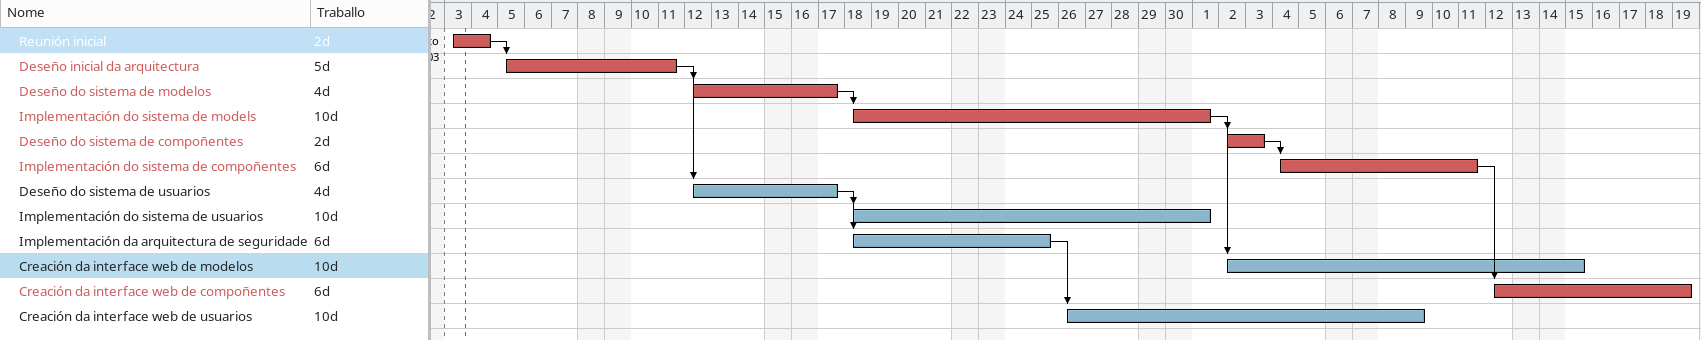
\includegraphics[width=\textwidth,width=50em]{imaxes/gantt.png}
	\caption{Diagrama de Gantt das fases do proxecto}
	\label{fig:gantt}
\end{figure}
\vspace*{5em}

Dentro do esquema de SPRINT definíronse 3 fases: modelo, compoñentes e usuarios. Dentro de cada fase incluíronse como incrementos as tarefas indicadas anteriormente.

\section{Orzamento}

A previsión do orzamento que pode precisar a realización dun proxecto depende de moitos factores únicos para cada empresa. Aquí preséntase unha posible aproximación, pensando no ambiente dunha empresa pequena. Hai dúas clases de custos: periódicos e únicos. Os custos periódicos son aqueles que se repiten cada certo tempo. Dentro deste ámbito incluiríanse os salarios dos traballadores ou as licenzas, se as houber. Os únicos corresponden á adquisición do material que precisa cada traballador, e ocorren ao inicio do proxecto.

Inda que o máis probable é que o persoal xa dispoña do material que precisa doutros proxectos, inclúese no cálculo. Para os ordenadores engadiuse un orzamento de 1000 € por desenvolvedor, e o IDE representa un custo de 724,79€ por desenvolvedor (para un ano). Isto representa 1724,79€ por desenvolvedor, e $ 10 348,74€ $.

O tamaño do equipo calcúlase en seis persoas como un tamaño óptimo\cite{chaosmanifesto}. Considerarase un salario medio anual de $ 36 000€ $\cite{ccii}\cite{confidencial}\cite{ine}. A duración dun proxecto de \textit{software} non é sinxelo de calcular, pero para este, considerando o tempo da realización deste traballo de fin de grao, escolléronse 3 meses para esta versión inicial. Isto daría un custo en salarios de $ 36000 ~ \sfrac{\text{€}}{\text{persoa} \cdot \text{ano}} \cdot 6 ~ \text{persoas} \cdot \frac{3 ~ \text{meses}}{12 ~ \tfrac{\text{meses}}{\text{ano}}} = 54000 € $ para os tres meses de desenvolvemento.

Isto representa un custo total de $ 64 348,74€ $
 \chapter{Tecnoloxías empregadas}
\label{chap:tecnoloxias}

As tecnoloxías empregadas foron:

\begin{itemize}
    \item Para ambas partes:
        \begin{itemize}
            \item Java
            \item Spring Boot
            \item Maven
            \item OpenAPI
            \item Docker
        \end{itemize}
    \item Só na parte de servidor:
        \begin{itemize}
            \item Hibernate/JPA
            \item Tomcat
            \item Jakarta RESTFull Web Services (JAX-RS)
            \item Swagger Codegen, para xerar a definición \Gls{openapi} a partir da interface JAX-RS
            \item JUnit5
            \item ANTLR4
        \end{itemize}
    \item Só na parte de cliente:
        \begin{itemize}
            \item Spring MVC
            \item Spring Security
            \item Swagger Codegen, para xerar un cliente REST a partir dunha definición \Gls{openapi}
            \item Thymeleaf
            \item Bootstrap
        \end{itemize}
    \item Ferramentas:
    	\begin{itemize}
    		\item IntelliJ
    		\item Git
    		\item Overleaf/TeXstudio e \LaTeX
    	\end{itemize}
\end{itemize}

A principal métrica á hora de buscar ferramentas foi a simplicidade na integración, buscando sempre a máxima automatización e evitando a repetición de código.

A linguaxe de programación Java foi escollida pola súa familiaridade, froito do seu uso continuado durante a carreira, especialmente durante as prácticas en empresa, onde tiven a oportunidade de empregar algunhas das tecnoloxías usadas neste proxecto: Spring e OpenAPI\cite{openapi}. Spring é un conxunto de bibliotecas que expanden Java de moitos xeitos distintos, aforrando traballo e automatizando moitas tarefas, por exemplo mediante a inxección de dependencias, que crea instancias de clases automaticamente con só definilas como parámetros dunha función ou construtor. Neste proxecto úsanse os módulos Spring Boot, que xestiona o ciclo de vida dunha aplicación; Spring MVC, que permite a creación de aplicacións usando a arquitectura Modelo-Vista-Controlador; e Spring Security, que xestiona a autenticación e autorización da aplicación mediante unha API adaptable.

Ambos os módulos están empaquetados en contedores Docker. Para reducir o tamaño dos contedores, estruturáronse en dúas etapas. A primeira etapa, baseada nun contedor base con maven e o JDK 17, encárgase de compilar o código e xerar o JAR resultante usando a orde \texttt{mvn package spring-boot:repackage}. A segunda etapa, baseada nun contedor base só co JRE 17, encárgase de coller o JAR da primeira etapa, copialo ao cartafol correcto e definir o punto de entrada do programa.

Un \texttt{compose.yml} na raíz do proxecto encárgase de xuntar e conectar os contedores de cada módulo. Xunto cun contedor de PostgreSQL, defínense 3 servizos divididos en dúas redes: unha para o «\textit{backend}», coa base de datos de PostgreSQL e o servizo \textit{pleste-server}, e outra para o «\textit{frontend}» cos servizos de \textit{pleste-server} e \textit{pleste-client}. Tamén se define un contedor para a base de datos de PostgreSQL. A creación dos dous contedores precisa facerse por separado, por mor de que \textit{pleste-client} precisa de conectarse a \textit{pleste-server} para descargar a definición de OpenAPI, pero o módulo de compilación usado por Docker non permite o acceso á rede, nin a definición de dependencias en tempo de compilación. Por isto, o primeiro que se fai é compilar e activar o contedor de \textit{pleste-server}:

\begin{lstlisting}[language=bash]
docker compose up -d pleste-server 
\end{lstlisting}

\newpage

Porén, inda que o servidor estea activo, precisa accederse dende o compilador en tempo de execución. Como o novo módulo de compilación de Docker non permite acceder a redes de Docker\cite{dockernetwork}, hai que forzar o uso do módulo de compilación antigo:

\begin{lstlisting}[language=bash]
DOCKER_BUILDKIT=0 docker compose build pleste-client
\end{lstlisting}

Outra solución sería modificar o \texttt{pom.xml} de \textit{pleste-client} para que faga conexión co servidor mediante a rede externa de Docker. Decidiuse deste outro xeito para depender o mínimo do entorno anfitrión.

\section{Servidor}
\label{sec:tec_servidor}

Para a parte do servidor úsase a plataforma de \textit{Jakarta RESTful Web Services} para implementar unha interface REST a partir dunha interface Java (referida neste caso ao conxunto de métodos públicos dunha clase) normal, aproveitándoa para xerar automaticamente o código para escoitar peticións HTTP, e chamar ás funcións axeitadas segundo o método e ruta da petición. Para automatizar a xeración de clientes, engadiuse tamén o xerador de OpenAPI, que permite xerar un documento JSON.

Para a API escolleuse HTTP con JSON pola súa simplicidade de funcionamento e integración con Jakarta, popularidade e transparencia. Isto permite, entre outras, comprobar o correcto funcionamento cun inspector de paquetes. HTTP é un protocolo cliente/servidor de nivel de aplicación que permite o intercambio de documentos  mediante o envío de mensaxes\cite{rfc9112}. Estas mensaxes conteñen cabeceiras en texto que definen os metadatos do corpo da mensaxe, se os houber. Para o cliente existen varios tipos de mensaxes, pero neste proxecto úsanse as mensaxes GET, POST, PUT e DELETE; cada mensaxe ten unha semántica distinta e unha serie de posibles respostas do servidor\cite{rfc7231}. Inda que orixinalmente orientado ao envío de documentos de texto, é posible usar eses mesmos verbos para crear interfaces remotas, usando JSON para o envío de datos estruturados dentro dos corpos das mensaxes.\cite{rest} A documentación da semántica de cada mensaxe e a súa resposta forma a especificación OpenAPI.\cite{jpaquery}

Para o almacenamento e xestión da información, úsase como base de datos relacional PostgreSQL. Para acceder á base de datos incluíuse o «\textit{framework}» \textit{Hibernate}, unha implementación da interface \acrshort{JPA} que permite xerar peticións SQL a partir de etiquetas en obxectos Java, xestionando tamén as sesións, creación e actualización das táboas, mediante unha interface \acrshort{CRUD}. Estas interfaces fan peticións sen precisar escribir código SQL, usando os nomes dos métodos nas interfaces para identificar que teñen que facer. Tampouco precisan unha clase que as implemente, abonda con usar Spring para inxectar as dependencias precisas. Para que sexa inda máis sinxelo, úsase unha clase \texttt{SQLDaoFactoryUtil} que, tamén mediante Spring, inicializase a si mesma e da acceso a todas as interfaces.

PostgreSQL é unha base de datos relacional, de código aberto e orientada aos ámbitos empresariais e para pequenos usuarios.\cite{postgres} Esta é unha base de datos axeitada para a carga de traballo pensada, e ademais permite unha escalabilidade que evitará que sexa un posible colo de botella no futuro. Pensouse en usar unha base de datos non relacional, especialmente á hora de modelar o polimorfismo nos campo dos compoñentes, pero rexeitouse por mor da súa complexidade e dificultade de integración co sistema xa montado en Hibernate.

Para xuntar \textit{Hibernate}, Jakarta e correr o servidor web que esta última precisa, incluíuse o «\textit{framework}» \textit{Spring Boot} con Tomcat, o servidor predeterminado en Spring. Ademais, \textit{Spring Boot} serve para realizar a inxección de dependencias.

Porén, o xeito de integrar Hibernate e os puntos REST nas mesmas clases de Java causa certas incompatibilidades e engadiu complexidade aos métodos responsables das peticións.

Os dous principais problemas relaciónanse por como Hibernate xestiona as claves foráneas. O primeiro é que Hibernate intenta reducir as peticións ás bases de datos e só inxectar os atributos cando se usen; ao serializar a JSON estas clases teñen os atributos como nulos e aparecen métodos «pantasma», que son os que inxectan os atributos pero que Jakarta non sabe serializar. O segundo é que, por omisión, serialízanse os atributos non primitivos como clases completas, o que é ineficiente se só se precisan algúns poucos atributos, ou mesmo só o ID.

Tamén engadíronse probas unitarias que comproban o funcionamento da parte servidor da aplicación, usando JUnit e integrando Spring para a inxección de dependencias. E realizáronse probas de integración de xeito manual, probando todas as funcionalidades da aplicación mediante un navegador web e CURL.

Para a parte de busca valoráronse 3 tecnoloxías: desenvolver un módulo de análise léxico e sintáctico propio, usar ANTLR\cite{antlr} ou JavaCC\cite{javacc}. Desenvolver un módulo propio descartouse pola súa complexidade e problemas que pode dar ante casos de uso pouco probables, pero que poderían amosar fallos en partes do código difíciles de probar pola gran cantidade de posibles entradas. Entre JavaCC e ANTLR, valorouse que ambas teñen integración con Maven. Porén, decidiuse usar ANTLR pola súa sintaxe para definir gramáticas, que é máis sinxela e seméllase máis á forma Backus-Naur, mentres que a sintaxe de JavaCC aseméllase máis á de Java.

Con ANTLR, tras xerar as clases axeitadas a partir da definición, existen dous xeitos de recorrer a árbore de sintaxe que crea\cite{visitor}: un \texttt{Listener}, e un \texttt{Visitor}. Ambos recorren a árbore en profundidade, pero de xeito distinto. Un \texttt{Listener} presenta unha interface con dous métodos por cada regra sintáctica, un que executa ao entrar na regra, e outro ao saír dela. Pola outra banda, un \texttt{Visitor} só ten un método por regra, que executa ao entrar na regra e que sae da regra ao devolver o método. Isto fai que o programador poida decidir se entrar ou non nos nodos fillo, e de que xeito.

\section{Cliente}

No cliente usáronse os «\textit{framework}» \textit{Spring Boot} e \textit{Spring MVC}. \textit{Spring Boot} forma a base da aplicación, que despois \textit{Spring MVC} aproveita para construír unha interface de usuario usando o patrón «\textit{\acrlong{MVC}}». No caso desta aplicación, a «Vista» corresponde coas páxinas web, que están ligadas a unhas clases «Controladoras» que son as que reciben as peticións HTTP e as procesan, chamando ao modelo segundo precisen.

Para facer a parte de «Modelo» usouse a mesma ferramenta de xeración de OpenAPI que a usada no servidor. Esta ferramenta permite que, unha vez configurado o enderezo do que obter o ficheiro \texttt{openapi.json}, recrear a interface Java do servidor coma se for unha dependencia máis de Maven, xestionando o xerador toda a parte de abrir a conexión HTTP, acceder ás rutas axeitadas e serializar e deserializar os obxectos de JSON a Java. Grazas a isto, o uso da API faise de xeito practicamente nativo, tendo algunhas dificultades á hora de traballar coas excepcións, que o xerador colapsa nunha clase \texttt{ApiException} da que despois hai que extraer os códigos de fallo correspondentes.

Para facer a interface con HTML usouse o motor de modelado Thymeleaf, que intégrase ben con Spring Boot. Para o deseño das páxinas incluíuse o «\textit{framework}» Bootstrap, principalmente a súa parte de CSS, para mellorar o deseño e adaptabilidade das páxinas.

\section{Autenticación e seguridade}
\label{sec:seguridade}

O sistema de seguridade baséase en dúas tecnoloxías distintas, unha no servidor e outra no cliente:

No caso do servidor, a seguridade proporciónaa Jakarta. Poderíase usar Spring Security tamén aquí, pero ao usar as etiquetas de Jakarta, Spring da problemas á hora de interceptar as peticións.

No lado do cliente, a seguridade é traballo de Spring Security. Este módulo encárgase de todo, dende interceptar as peticións, redirixir á páxina de inicio de sesión e, se se aproveitan as clases incluídas no módulo, almacenar credenciais, autenticalas e autorizalas sen ter que escribir código propio.

Isto explícase máis detallado no capítulo \ref{chap:seguridade}.

\newpage

\section{Ferramentas}
\label{sec:ferramentas}

Neste traballo usáronse varias ferramentas non mencionadas anteriormente:

\subsection{IntellIJ}

Escolleuse o IDE de IntelliJ pola sua completitude e integración, non só coa linguaxe Java, se non tamén coas bibliotecas de Spring, Hibernate, JUnit, Jakarta e Thymeleaf.\cite{intellij}ç

\subsection{Git}

Como sistema de control de versións escolleuse Git, e especialmente a plataforma de GitHub para gardar o proxecto. Git é practicamente o único sistema de control de versións, polo que a súa elección foi sinxela. Escolleuse a plataforma de GitHub por estar xa integrada co correo corporativo doutras materias previas.

\subsection{Overleaf/TeXstudio e \LaTeX}

O deseño da memoria baseouse no modelo en \LaTeX da Facultade. Usouse tanto a plataforma de Overleaf como, cando esta non funcionaba, o programa TeXstudio.
 \chapter{Deseño}
\label{chap:deseno}

\section{Análise de requisitos}

A primeira fase foi recoller requisitos e a delineación do dominio do problema a resolver. Para isto realizouse unha reunión inicial cos co-directores do traballo para entender as casuísticas das que nace a necesidade deste traballo. Despois de varias reunións cos co-directores, chegouse aos seguintes casos de uso (véxase diagrama \ref{fig:casosuso}):

\subsection{CU-01: Xestionar modelos}

Da xestión de modelos encárganse os actores Administradores, o que inclúe creación, borrado e modificación.

\subsection{CU-02: Ver modelos}

Ver os modelos inclúese separado de xestionalos, por que é a única acción que pode facer un técnico sobre os modelos; ademais, precísao para poder crear os compoñentes.

\subsection{CU-03: Xestionar compoñentes}

A xestión de compoñentes pode realizarse indistintamente polos actores Técnicos e Administradores, creación, borrado, visualización e modificación.

\subsection{CU-04: Xestionar usuarios}

A xestión de usuarios é exclusiva dos administradores.

\begin{figure}
	\hspace*{-3cm}
	\centering
	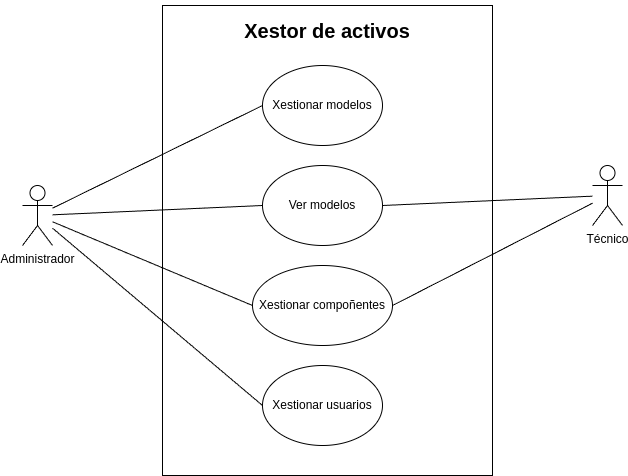
\includegraphics[width=0.7\textwidth]{imaxes/casos_uso.drawio.png}
	\caption{Diagrama de casos de uso}
	\label{fig:casosuso}
\end{figure}

\section{Esquema do sistema}

A plataforma está formada por dous tipos de obxectos: modelos (\Gls{Template}) e compoñentes (\Gls{Component}). Tamén hai dous tipos de usuarios: administradores e técnicos.

\section{Obxectos}

A primeira versión da aplicación presentaba unha serie de obxectos concretos, tales coma servidores ou programas. Porén, tras falar cos codirectores e ver un chisco o uso real por parte de técnicos, escolleuse facer un sistema máis xenérico, que permita adaptarse ás necesidades de cada ambiente. O obxectivo é que cada técnico poida usar a aplicación do xeito que máis se axuste ao seu traballo. A figura \ref{fig:erobxectos} amosa a relación entre os distintos obxectos do sistema.

\subsection{Modelos}

Os modelos representan unha clase de compoñentes. Están formados por campos, e a súa creación correspóndelle aos administradores. Cada campo do modelo deberá indicar se se trata de texto libre, dunha ligazón a unha entidade ou dunha data. As ligazóns deberan apuntar a un compoñente.

\newpage

Dentro da aplicación inclúense algúns modelos predefinidos:

\begin{itemize}
    \item Ordenador
    \item Programa
    \item Licenza
\end{itemize}

Para evitar inconsistencias, non se poden modificar os campos dos modelos se xa teñen compoñentes asociados.

\subsection{Compoñente}

Os compoñentes corresponden a instancias individuais de modelos. Ao crear un compoñente deberanse encher tamén os campos correspondentes. As entidades, segundo se indique no seu modelo correspondente, poden ligarse entre si: ao visualizar unha entidade tamén se poden consultar as entidades que ligan a, e dende, esta.

\section{Usuarios}
\label{sec:usuarios}

\subsection{Administradores}

Os administradores son os usuarios encargados da creación dos modelos para que usen os técnicos. Tamén poderán encargarse da xestión e rexistro de usuarios.

\subsection{Técnicos}

Os técnicos son os usuarios que xestionan os compoñentes, e encárganse de manter actualizada a base de datos durante o transcurso do seu labor.


\begin{figure}
    \centering
    \resizebox{.8\linewidth}{!}{\digraph{"Diagrama esquema-relación"}{
layout=neato;

node [colorscheme = ylgnbu4, shape = none, margin = 0];
edge [colorscheme = dark28, dir = both];

node [shape=box];
	Usuarios;
	Modelos;
	Compoñentes;
	Campos[peripheries=2];
	Datos[peripheries=2];
node [shape=ellipse];
	{node [label="nome"] nome0[label=<<U>nome</U>>]; nome1; nome2[label=<<U>nome</U>>]; nome3[label=<<U>nome</U>>];};
	{node [label="descripción"] descripcion0; descripcion1;};
	contrasinal; rol;
	tipo; contido;
	id[label=<<U>id</U>>];
node [shape=diamond,style=filled,color=lightgrey];
	CD[label="Contén",peripheries=2,color=""];
	MCa[label="Contén",peripheries=2,color=""];
	MC[label="Baseados en"];
	DC[label="Ligazón a"];
	UM[label="Crea e modifica"];
	UC[label="Crea e modifica"];
	CaD[label="Deriva de",peripheries=2,color=""];

Modelos -> MCa [label="1",len=1.25,arrowhead=none,arrowtail=none];
MCa -> Campos [label="n",len=1.50,arrowhead=none,arrowtail=none,color="black:black"];

Modelos -> MC [label="n",len=1.50,arrowhead=none,arrowtail=none];
MC -> Compoñentes [label="1  ",len=1.50,arrowhead=none,arrowtail=none,color="black:black"];

Compoñentes -> CD [label="1  ",len=1.50,arrowhead=none,arrowtail=none];
CD -> Datos [label="n",len=1.50,arrowhead=none,arrowtail=none,color="black:black"];

Datos -> DC [label="n",len=2.00,arrowhead=none,arrowtail=none];
DC -> Compoñentes [label="m",len=2.00,arrowhead=none,arrowtail=none];

Campos -> CaD [label="1     ",arrowhead=none,arrowtail=none];
CaD -> Datos [label="n",arrowhead=none,arrowtail=none,color="black:black"];

Usuarios -> UM [label="n",len=1.50,arrowhead=none,arrowtail=none];
UM -> Modelos [label="m",len=1.50,arrowhead=none,arrowtail=none,color="black:black"];
Usuarios -> UC [label="n",len=1.50,arrowhead=none,arrowtail=none];
UC -> Compoñentes [label="m",len=1.50,arrowhead=none,arrowtail=none,color="black:black"];

nome0 -> Usuarios[arrowhead=none,arrowtail=none];
nome1 -> Compoñentes[arrowhead=none,arrowtail=none];
nome2 -> Modelos[arrowhead=none,arrowtail=none];
nome3 -> Campos[arrowhead=none,arrowtail=none];

descripcion0 -> Modelos[arrowhead=none,arrowtail=none];
descripcion1 -> Compoñentes[arrowhead=none,arrowtail=none];

id -> Compoñentes[arrowhead=none,arrowtail=none];

contrasinal -> Usuarios[arrowhead=none,arrowtail=none];
rol -> Usuarios[arrowhead=none,arrowtail=none];

tipo -> Campos[arrowhead=none,arrowtail=none];
contido -> Datos[arrowhead=none,arrowtail=none];
}}
    \caption{Diagrama Esquema-Relación dos obxectos do sistema}
    \label{fig:erobxectos}
\end{figure}

\section{Busca}

A busca realízase mediante unha serie de comparacións entre propiedades e valores, unidas mediante operacións lóxicas.

As propiedades serán da forma «\textit{obxecto}.\textit{atributo}». Os obxectos serán os indicados na sección anterior. Os atributos poderán ser calquera dos indicados na figura \ref{fig:erobxectos}. Poderán compararse os contidos e atributos dos campos de compoñentes e modelos usando a mesma sintaxe de atributos separados por puntos. A propiedade que representa o valor dos campos é especial, e, dependendo da operación, só coincidirá con certos tipos de campos.

Para detalles máis específicos, véxase a sección \ref{sec:busca}.

Existen tres grupos de operacións a realizar: sobre cadeas, sobre números e sobre conxuntos.

As operacións sobre cadeas realizan unha comparación usando expresións regulares Para a comparación úsanse os operadores \textasciitilde e !\textasciitilde para a versión negada. A operación sobre cadeas pódese usar sobre todas as propiedades; se se aplica sobre o valor dos campos só coincidirá en campos de tipo texto ou data (neste caso sobre a representación textual da data). Esta operación pode usarse sobre todas as propiedades, e no caso do valor dos campos sobre os de tipo cadea e data (neste caso sobre a representación textual das mesmas).

As operacións sobre conxuntos son equivalentes a realizar unha serie de operacións sobre cadeas, unidas por disxuncións lóxicas. Úsanse coma operadores «@» ou «!@» (versión negada), e seguido unha listaxe de cadeas entre corchetes separadas por comas. Deste xeito, \texttt{template.name @ [ "A", "B", "C" ]} é equivalente a facer \texttt{template.name \textasciitilde "A" | template.name \textasciitilde "B" | template.name \textasciitilde "C"} Esta operación pode usarse sobre as mesmas propiedades ca as sobre cadeas, e tamén nos valores dos campos de tipo numérico e ligazóns, que deberán ser números completos e non expresións regulares.

As operacións sobre números aplícanse exclusivamente ao valor de campos, e só aos de tipo número, data e ligazón. As condicións posibles serán de maior (ou igual) que, menor (ou igual) que, igual ou non igual. Nas datas compararase se o valor é posterior ou anterior á data indicada. Para as ligazóns só se poderán usar as condicións de igualdade ou non igualdade.

\newpage

As operacións lóxicas son a conxunción (co operador «\&») e a disxunción (co operador «|»). Ambas operacións teñen a mesma precedencia e asócianse de esquerda a dereita, de xeito que \texttt{a | b \& c} é o mesmo que \texttt{ (a|b) \& c }. Pódense usar parénteses para indicar a precedencia.

Isto da coma resultado a seguinte gramática independente do contexto en forma Backus–Naur:

\begin{grammar}
	<expresión> ::= <proba>
	\alt '(' <expresión> ')'
	\alt <expresión> '\&' <expresión>
	\alt <expresión> '|' <expresión>
	
	<proba> ::= <propiedade> ( `~' | `!~' ) <cadea>
	\alt <propiedade> ( `>=' | `<=' | `>' | `<' | `=' | `!=' ) ( <número> | <data> )
	\alt <propiedade> ( `@' | `!@' ) `[' <cadea> (',' <cadea>)* `]'
\end{grammar}

Os elementos terminais defínense usando expresións regulares. \texttt{<número>} defínese coma un número racional ([+-]?[0-9]+\allowbreak{}(\.[0-9]+)?), \texttt{<cadea>} defínese coma calquera número de caracteres entre comiñas sen escapar (\verb|[^\]".*[^\]"|) e \texttt{<data>} defínese usando o formato ISO 8601\footnote{UNE-EN 28601:1995 na normativa española\cite{iso8601}} para data e hora sen incluír fuso horario ([0-9][0-9][0-9][0-9]-\allowbreak{}[0-9][0-9]-\allowbreak{}[0-9][0-9]T\allowbreak{}[0-9][0-9]:\allowbreak{}[0-9][0-9]:\allowbreak{}[0-9][0-9]).

Para a interpretación defínense dúas gramáticas: unha para a análise léxica e a outra para a análise sintáctica.

Na análise léxica defínese un alfabeto que inclúe todos os caracteres Unicode, limitado únicamente polos caracteres que acepta Java e PostgreSQL para cadeas. Sobre este alfabeto defínense certas linguaxes regulares: as xa indicadas previamente para definir números racionais, datas e cadeas; xunto coas que aceptan os operadores, comas, parénteses e corchetes.\footnote{Non se definen estas últimas pola súa simplicidade}. A definición da gramática que acepta propiedades sería

\begin{eqnarray}
l \in \{ a,b,c,d,e,f,g,i,j,k,l,m,n,ñ,o,p,q,r,s,t,u,v,w,x,y,z \} \\
p = l^{\ast}(.l^{\ast})^{\ast} 
\end{eqnarray}

\newpage

Na análise sintáctica defínese un alfabeto baseado no resultado da análise léxica:

\begin{equation}
\begin{gathered}
\Sigma = \{ \text{propiedade}, \text{comparación}, \text{non comparación}, \\
	\text{maior que}, \text{menor que}, \text{maior ou igual que}, \\
	\text{menor ou igual que}, \text{igual que}, \text{non igual que}, \\
	\text{en conxunto}, \text{non no conxunto}, \text{paréntese aberto}, \\
	\text{paréntese pechado}, \text{corchete aberto}, \text{coma} \\
	\text{corchete pechado}, \text{cadea}, \text{número}, \text{data}, \text{conxunción}, \text{disxunción} \}
\end{gathered}
\end{equation}

Entre o paso léxico e sintáctico elimináronse os espazos en branco, saltos de liña ou calquera outros caracteres que non afectan á sintaxe, execepto dentro de cadeas.

Como nesta gramática existen producións con varias expresións non terminais, precísase pasar dunha gramática regular a unha independente do contexto, e deste xeito poder usar operacións de conxunción e disxunción dunha forma moito máis lexible. Se non, habería que usar algunha notación prefixo ou limitar moito que tipo de comparacións poderíanse facer.\cite{teoria_automatas}

A modo de exemplo, vaise converter a cadea «\textit{(user.name @ ["root", " 12 "] \& user.role !@ [ "NORMAL" ]) | template.name \textasciitilde "y" \& template.name @ [ "A" ] \& component.field.value > 2}». Primeiro divídese mediante análise léxica, ignorando os espazos en branco:

\begin{eqnarray}
\underset{\text{paréntese aberto}}{(} \underset{\text{propiedade}}{user.name} \underset{\text{en conxunto}}{@} \underset{\text{corchete aberto}}{[} \underset{\text{cadea}}{"root"} \underset{\text{coma}}{,} \underset{\text{cadea}}{" 12 "} \underset{\text{corchete pechado}}{]} \underset{\text{conxunción}}{\&} \\
\underset{\text{propiedade}}{user.role}\underset{\text{non no conxunto}}{!@} \underset{\text{corchete aberto}}{[} \underset{\text{cadea}}{"NORMAL"} \underset{\text{corchete pechado}}{]} \underset{\text{paréntese pechado}}{)} \underset{\text{disxunción}}{|} \underset{\text{propiedade}}{template.name} \\
\underset{\text{comparación}}{\textasciitilde} \underset{\text{cadea}}{"y"} \ldots
\end{eqnarray}

A partir disto xerase a árbore de sintaxe (figura \ref{fig:arboresintaxe}):

\begin{figure}[H]
	\centering
	\resizebox{.8\linewidth}{!}{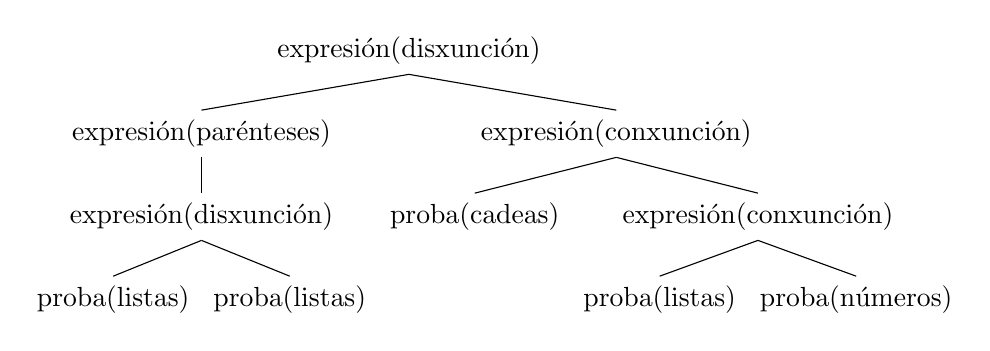
\begin{tikzpicture}
\Tree [.expresión(disxunción)
	[.expresión(parénteses)
		[.expresión(disxunción)
			proba(listas)
			proba(listas)
		]
	]
	[.expresión(conxunción)
		proba(cadeas)
		[.expresión(conxunción)
			proba(listas)
			proba(números)
		]
	]
]
\end{tikzpicture}}
	\caption{Árbore de sintaxe de exemplo}
	\label{fig:arboresintaxe}
\end{figure}
 \chapter{Interface gráfica}
\label{chap:gui}

A interface gráfica está estruturada coma unha páxina web. Cada ruta representa unha funcionalidade diferente, primando a simplicidade e lixeireza das páxinas web fronte a unha interactividade excesiva, típica dunha \acrshort{SPA}.

Aparte da páxina de inicio (ver figura \ref{fig:inicio2}), existen 12 páxinas principais: 4 por cada tipo de compoñente. Estas son:\footnote{Non se intentou seguir ningunha arquitectura ao deseñar as rutas das páxinas, ao considerarse un detalle interno de implementación}

\begin{itemize}
	\item Para os modelos:
	\begin{itemize}
		\item /newtemplate (figura \ref{fig:creart})
		\item /edittemplate?id=(id do modelo) (mesmo deseño ca \texttt{/newtemplate}, pero cos campos xa con texto)
		\item /managetemplates (figura \ref{fig:mt})
		\item /displaytemplate?id=(id do modelo)
	\end{itemize}
	\item Para os compoñentes:
	\begin{itemize}
		\item /newcomponent?template=(id do modelo base) (figura \ref{fig:crearc})
		\item /editcomponent?id=(id do compoñente) (mesmo deseño ca \texttt{/newcomponent}, pero cos campos xa con texto)
		\item /managecomponents (figura \ref{fig:mc})
		\item /displaycomponent?id=(id do compoñente) (figura \ref{fig:creadoc2})
	\end{itemize}
	\item Para os usuarios:
	\begin{itemize}
		\item /newuser (figura \ref{fig:crearu})
		\item /edituser?id=(id do usuario) (mesmo deseño ca \texttt{/newuser}, pero cos campos xa con texto)
		\item /manageusers (figura \ref{fig:mu})
		\item /displayuser?id=(id do usuario) (figura \ref{fig:creadou})
	\end{itemize}
\end{itemize}

Pódese acceder a calquera desas rutas mediante os botóns que se atopan en todas as páxinas. Ademais, a cabeceira da páxina contén un menú despregable que permite saltar rapidamente ás seccións importantes.

Por suposto, antes de poder acceder á aplicación en si é preciso iniciar sesión. Pódese ver na figura \ref{fig:login} como é a pantalla de inicio de sesión.

\section{Funcionamento de \textit{Spring MVC}}

No contexto de Spring MVC, os tres compoñentes implantase de xeito totalmente distinto:

\subsection{Modelo}

A parte de modelo é completamente interna a Spring. Este módulo encárgase de crear os obxectos asociados ao modelo, pasándoos aos compoñentes que precisen automaticamente.

\subsection{Vista}

Nesta parte é onde se aplica o sistema de modelado Thymeleaf. Para usalo, engádese o espazo de nomes de Thymeleaf á páxina que se vai usar. As páxinas HTML créanse no cartafol \texttt{resources/templates}. Thymeleaf permite incluír a información do modelo dentro da páxina, accedendo á información dentro duns atributos especiais, ademais de permitir usar construcións típicas de linguaxes de programación, como poden ser as condicións e os bucles. Amósase coma exemplo a páxina de inicio da aplicación:

\begin{lstlisting}[language=HTML]
<!DOCTYPE HTML>
<html xmlns:th="http://www.thymeleaf.org" lang="gl">
\end{lstlisting}

Thymeleaf precisa de incluír este espazo de nomes para poder usar os seus atributos propios

\newpage

\begin{lstlisting}[language=HTML]
<head>
<title>pleste: PLataforma de xEstión de configuraciónS TÉcnicas</title>
<meta http-equiv="Content-Type" content="text/html; charset=UTF-8" />
<th:block th:insert="~{includes}" />
</head>
<body>
<header th:insert="~{header}"></header>
\end{lstlisting}

Thymeleaf permite incluír outras páxinas, e deste xeito reutilizar elementos comúns usando o atributo \texttt{insert}.

\begin{lstlisting}[language=HTML]
<main class="container mt-5">
<a class="btn btn-info" role="button" href="/newtemplate">Crear un novo modelo</a>
<h2>Modelos xa creados</h2>
<ul>
<li th:each="template: ${templates}"><a th:href="|/template?id=${template.id}|" th:text="|Modelo ${template.name} (nº ${template.id})|"></a></li>
</ul>
</main>
</body>
</html>
\end{lstlisting}

Nesta sección inclúese un bucle. O bucle defínese usando o atributo \texttt{each}, que inclúe o nome do elemento iterado e, usando a sintaxe para acceder ao modelo (\texttt{\$\{atributo\}}), a lista. Con isto, Thymeleaf repetirá ese elemento HTML tantas veces coma elementos conteña a lista, asignando o valor á variable \texttt{template}. Para que a etiqueta \texttt{<a>} poida usar os valores da variable, precísanse engadir os campos propios de Thymeleaf, co prefixo \texttt{th:}, para que poida substituír o contido entre corchetes polo valor da propiedade dentro do obxecto.

\subsection{Controlador}

O controlador é onde está toda a lóxica da interface, e é o encargado de engadir os datos precisos ao Modelo. Dentro de Spring, para crear un controlador só se precisa crear unha clase, etiquetala con \texttt{@Controller}, e engadir os métodos que procesarán as peticións. Cada método deberá etiquetarse co tipo de petición e ruta que procesa, usando a etiqueta \texttt{@GetMapping("/")} (para procesar \texttt{GET}) ou \texttt{@PostMapping("/")} (para procesar \texttt{POST}). No cliente, todas as clases no cartafol \texttt{view} son controladores. Son estas clases as que realizan as chamadas á API REST, procesan os resultados e lanzan as excepcións.

Despois, a definición de cada método indicará de que xeito vai procesar a petición. Devolver unha cadea de texto indica que a cadea conterá o nome do ficheiro HTML a usar na vista, pero tamén se pode devolver unha clase \texttt{Model} ou \texttt{ModelView}, que permiten devolver directamente o modelo, pasando o ficheiro no construtor da clase, ou incluso calquera outra resposta, devolvendo un \texttt{ResponseEntity} creado co código, corpo e cabeceiras que se precisen. Dependendo dos parámetros da función, Spring pasaralle os obxectos que se precisen, dende o modelo (pasando unha clase \texttt{Model} ou \texttt{ModelView}) ou a sesión (clase \texttt{HttpSession}) ate os parámetros GET e POST da petición. Neste último caso, precisa que os parámetros sexan de tipo \texttt{String}, e que estean etiquetados con \texttt{@RequestParam}.

De xeito especial, pódese poñer un parámetro de tipo \texttt{Map<String, String>}, que conterá todos os parámetros da petición.

Para amosar o funcionamento da interface, vaise amosar exemplo de uso típico:

\section{Caso de uso: Creación dun novo compoñente}

Para este caso de uso de exemplo, vaise crear un novo compoñente rato, vinculado a un ordenador.

O primeiro paso é crear o ordenador. Para isto aprovéitase o modelo xa creado «Ordenador». A partir deste modelo créase o compoñente «PC-02», tal coma se pode ver nas figuras \ref{fig:crearc} e \ref{fig:creadoc}.

Despois vaise engadir un rato e vinculalo ao ordenador. Para isto créase o modelo «Rato» (figura \ref{fig:creart}), a partir do cal créase un compoñente rato (figura \ref{fig:crearc2}), e engádese nun campo unha ligazón ao compoñente «PC-02», como se pode ver no campo PC da figura \ref{fig:creadoc2}.

\newpage

\section{Galería de imaxes}

\newcommand*{\crearimaxe}[3][width=\textwidth]{
	\begin{figure}[htbp]
		%\hspace*{-3cm}
		\centering
		\frame{\includegraphics[#1]{imaxes/#2.png}}
		\caption{#3}
		\label{fig:#2}
		\centering
	\end{figure}
}

\vspace*{5em}
\crearimaxe[width=30em]{crearc}{Creando o compoñente «PC-02»}
\crearimaxe[width=0.9\textwidth]{creadoc}{Compoñente «PC-02» creado}
\crearimaxe[width=0.9\textwidth]{creart}{Creando o modelo «Rato»}

\crearimaxe[width=27em]{crearc2}{Creando o compoñente «Rato»}
\crearimaxe[width=27em]{creadoc2}{Compoñente «Rato» creado}

\crearimaxe[width=0.9\textwidth]{inicio}{Menú de inicio, antes de crear o modelo «Rato»}
\crearimaxe[width=0.9\textwidth]{inicio2}{Menú de inicio, co submenú aberto}

\crearimaxe{login}{Formulario de inicio de sesión}
\crearimaxe{mc}{Páxina de xestión de compoñentes}

\crearimaxe{mt}{Páxina de xestión de modelos}
\crearimaxe{mu}{Páxina de xestión de usuarios}

\crearimaxe[width=0.9\textwidth]{creadou}{Modificar un usuario}
\crearimaxe[width=0.9\textwidth]{crearu}{Engadir un novo usuario}

\crearimaxe{buscar}{Buscando un modelo}
\crearimaxe{buscarh}{Fragmento da páxina de axuda á busca}
 \chapter{Arquitectura}
\label{chap:arquitectura}

A plataforma está formada por dous compoñentes: unha parte servidor, implementada en Java e que realiza as labores de conexión coa base de datos, e que presenta unha \acrshort{API} \acrshort{REST} ao exterior; e unha parte cliente, un servidor Web en Java que conecta á parte servidor mediante peticións á \acrshort{API} \acrshort{REST}. Decidiuse engadir unha API REST, e non só integrar todo no mesmo sistema, para permitir futuras extensións e aplicacións alternativas, que permita un acceso máis cómodo e adaptado ao persoal técnico. O esquema de deseño fundamental foi «\textit{API first}», pensando en presentar un mesmo método de interacción mediante peticións HTTP con JSON, no canto de integrar o cliente dentro da aplicación e que chamar directamente aos métodos dende Java.

\section{Obxectos}

Existen cinco obxectos principais. A figura \ref{fig:diagrama_clases} representa as relacións entre as clases:

\subsection{Template}
\label{obx:template}

Representa un modelo a partir do cal sacar \Gls{Component}.

\textbf{Campos:}

\begin{description}
    \item[id] Valor numérico que representa o ID do modelo
    \item[name] Cadea que contén o nome do modelo
    \item[description] Cadea que conten unha pequena descrición do modelo
    \item[fields] Lista de clases \Gls{TemplateField}, que son os campos do modelo
\end{description}

\subsection{Component}
\label{obx:component}

Representa un compoñente creado a partir dun \Gls{Template}.

\textbf{Campos:}

\begin{description}
    \item[id] Valor numérico que representa o ID do compoñente
    \item[name] Cadea que contén o nome do compoñente
    \item[description] Cadea que conten unha pequena descrición do compoñente
    \item[template] Clave foránea/punteiro que apunta ao \Gls{Template} do que se creou este Component
    \item[fields] Lista de clases \Gls{Field}, que son os campos do compoñente
\end{description}

\subsection{TemplateField}
\label{obx:tfield}

Representa os campos do modelo, que son a base para crear os campos do \Gls{Component}.

\textbf{Campos:}

\begin{description}
    \item[id] Valor numérico que representa o ID do campo
    \item[name] Cadea que contén o nome do campo. Non se poden repetir no mesmo \Gls{Template}
    \item[mandatory] Valor binario que indica se o campo é obrigatorio
    \item[type] Indica o tipo do campo con un enumerado.
\end{description}

Os tipos de campos son:

\begin{description}
    \item[\texttt{TEXT}] Permite gardar texto plano e sen formato
    \item[\texttt{LINK}] Representa unha ligazón a outro compoñente
    \item[\texttt{DATETIME}] Representa unha data
\end{description}

\subsection{Field}
\label{obx:field}

Representa un campo dun \Gls{Component}.

\textbf{Campos:}

\begin{description}
    \item[id] Valor numérico que representa o ID do campo
    \item[type] Tipo do campo, copiado do \Gls{TemplateField} e usado para diferenciar durante a serialización
    \item[content] Atributo «virtual», que serve para indicarlle a OpenAPI que clases poden conterse dentro do campo.
    \item[templateField] Ligazón/clave foránea no modelo relacional ao campo do \Gls{Template} no que se basea este campo o \Gls{Component} 
\end{description}

O obxecto \texttt{Field} é unha clase abstracta, e parametrizada cunha clase xenérica que serve para devolver distintos tipos de obxectos. Para poder usar herdanza na base de datos hai tres tipos de estratexias:\cite{herdanza}

\begin{itemize}
	\item \texttt{MappedSuperclass}, que crea unha táboa por cada subclase (pero non para a superclase) replicando todas as columnas herdadas e propias. O problema que ten isto é que non se pode referenciar á superclase dende outras táboas da base de datos, o que neste caso impediría que \texttt{Component} tivera unha foránea a \texttt{Field}, e tería que ter foráneas a todos os campos individuais.
	\item Reunir nunha soa táboa todas as subclases. Isto permite engadir foráneas, pero o número de subclases e o rendemento están limitados polo número de columnas que acepte a base de datos.
	\item Unha táboa por subclase, de xeito que para acceder a unha entidade precísase facer unha operación de \texttt{JOIN} entre a táboa da subclase e da superclase. Non ocupa tanto espazo coma a seguinte opción, pero é máis lenta ca a anterior opción por mor de precisar acceder a varias táboas.
	\item Unha táboa completa por subclase, tendo cada táboa da subclase os seus atributos máis os da superclase. Non se precisan facer \texttt{JOIN}, pero ocupa máis espazo ao ter que duplicar todos os atributos.
\end{itemize}

Escolleuse a 2ª opción por ser a máis sinxela, eficiente e ser a opción predeterminada en Jakarta. Ademais, non se considera que o número de tipos de campos vaia medrar dabondo coma para ser un problema. E, en calquera caso, poderíase migrar a calquera das outras opcións só cambiando unha anotación.

As subclases existentes son:

\begin{description}
    \item[\texttt{TextField}] Representa un campo de texto. Substitúe a clase xenérica por unha clase \texttt{String}
    \item[\texttt{DatetimeField}] Representa un campo de texto. Substitúe a clase xenérica por unha clase \texttt{JSONDatetime}
    \item[\texttt{LinkField}] Representa unha ligazón a outro compoñente.  Substitúe a clase xenérica por unha clave foránea a unha clase \texttt{Component}
    \item[\texttt{NumberField}] Representa un valor numérico decimal. Substitúe a clase xenérica por \texttt{BigDecimal}
\end{description}

Inda que cada subclase ten unha propiedade \texttt{content} distinta para evitar colisións na base de datos, o contido é o mesmo.

\subsection{User}
\label{obx:user}

Representa un usuario no sistema.

\textbf{Campos:}

\begin{description}
    \item[id] Valor numérico que representa o ID do usuario
    \item[username] Cadea que contén o alcume do usuario
    \item[email] Cadea que contén o enderezo electrónico do usuario
    \item[password] Cadea que contén o contrasinal do usuario, cifrado con \Gls{BCrypt}
    \item[role] Enumerado que contén o tipo de rol do usuario
\end{description}

Os posibles valores para o campo role son \texttt{ADMINISTRATOR} e \texttt{NORMAL\_USER}. Para máis información, consulte a sección \ref{sec:usuarios}.

Para os usuarios tamén existe a clase Token, que, aparte do usuario ao que referencia e un ID, garda unha \Gls{testemuna} nunha cadea.

\begin{figure}\hspace*{-3cm}
    \centering
    \resizebox{.9\textwidth}{!}{\begin{tikzpicture}
\begin{class}{Template}{20,0}
	\attribute{id : long}
	\attribute{name : String}
	\attribute{description : String}
	\attribute{fields : TemplateField[0..*]}
\end{class}
\begin{class}{TemplateField}{10,0}
	\attribute{id : long}
	\attribute{name : String}
	\attribute{mandatory : boolean}
	\attribute{type : FieldTypes}
\end{class}
\begin{class}{FieldTypes}{0,0}
	\attribute{TEXT}
	\attribute{DATETIME}
	\attribute{LINK}
	\attribute{NUMBER}
\end{class}

\composition{Template}{0..*}{fields}{TemplateField}
\aggregation{TemplateField}{1}{type}{FieldTypes}

\begin{class}{Component}{17,5}
	\attribute{id : long}
	\attribute{name : String}
	\attribute{description : String}
	\attribute{fields : Field[0..*]}
	\attribute{template : Template}
\end{class}
\begin{abstractclass}[template=T]{Field}{8,7}
	\attribute{id : long}
	\attribute{type : FieldTypes}
	\attribute{templateField : TemplateFields}
	\attribute{content : T}
	\operation{getContent() : T}
	\operation{setContent(content : T) }
\end{abstractclass}
\begin{class}{NumberField}{0,10}
	\inherit{Field}
	\attribute{number\_content : BigDecimal}
	\operation{getContent() : BigDecimal}
	\operation{setContent(content : BigDecimal)}
\end{class}
\begin{class}{TextField}{8,10}
	\inherit{Field}
	\attribute{text\_content : String}
	\operation{getContent() : String}
	\operation{setContent(content : String)}
\end{class}
\begin{class}{DatetimeField}{0,6}
	\inherit{Field}
	\attribute{datetime\_content : JSONDatetime}
	\operation{getContent() : JSONDatetime}
	\operation{setContent(content : JSONDatetime)}
\end{class}
\begin{class}{LinkField}{15,10}
	\inherit{Field}
	\attribute{link\_content : Component}
	\operation{getContent() : Component}
	\operation{setContent(content : Component)}
\end{class}

\composition{Component}{0..*}{fields}{Field}
\unidirectionalAssociation{LinkField}{1}{link\_content}{Component}
\aggregation{Field}{1}{type}{FieldTypes}
\aggregation{Component}{1}{template}{Template}
\aggregation{Field}{1}{templateField}{TemplateField}

\begin{class}{User}{7,15}
	\attribute{id : long}
	\attribute{username : String}
	\attribute{email : String}
	\attribute{password : String}
	\attribute{role : Roles}
\end{class}
\begin{class}{Token}{0,15}
	\attribute{id : long}
	\attribute{user : User}
	\attribute{token : String}
\end{class}
\begin{class}{Roles}{15,15}
	\attribute{NORMAL\_USER}
	\attribute{ADMINISTRATOR}
\end{class}


\aggregation{User}{1}{role}{Roles}
\aggregation{Token}{1}{user}{User}

\end{tikzpicture}}
    \caption{Diagrama de clases do servidor}
    \label{fig:diagrama_clases}
\end{figure}

\section{API REST do servidor}

Todas as rutas que inclúen algún id ou nome, devolven un «\textit{HTTP 404 Not Found}» se non existe algún dos identificadores ou nomes. A API acepta tanto JSON coma XML, pero o cliente só usa JSON.

A meirande parte das peticións precisan dunha testemuña válida pasa na cabeceira «\texttt{X-API-KEY}». Para máis información sobre permisos consultar a sección 
\ref{sec:seguridade}

Todas as rutas descritas son relativas á ruta \texttt{\$SERVIDOR/api/v0/\$SUBSECCIÓN}.

\newpage

\subsection{\texttt{/templates}}

Nesta sección xestiónanse os modelos os seus campos.

\texttt{/}

\begin{description}
    \item[GET] Devolve unha listaxe de todos os modelos dispoñibles. Permite devolver só un rango engadindo os parámetros \texttt{skip} e \texttt{count}
    \item[POST] Crea un novo modelo incluído no corpo da petición. Devolve un «\textit{HTTP 409 CONFLICT}» se xa existe outro modelo co mesmo nome
\end{description}

\texttt{/find?name=(nome)}

\begin{description}
    \item[GET] Devolve unha listaxe de todos os modelos dispoñibles cuxo nome coincide con «nome»
\end{description}

\texttt{/(id)}

\begin{description}
    \item[GET] Devolve o modelo con id \texttt{id}
    \item[POST] Actualiza o modelo co contido do corpo da petición
    \item[DELETE] Elimina o modelo. Devolve un HTTP 409 Bad Request se inda quedan \Gls{Component}s vinculados a este modelo
\end{description}

\texttt{/(id)/components}

\begin{description}
    \item[GET] Devolve unha listaxe de todos os compoñentes derivados deste modelo
\end{description}

\texttt{/(id)/fields}

\begin{description}
    \item[GET] Devolve unha listaxe de todos os campos deste modelo
    \item[POST] Engade un novo campo ao compoñente. Falla se o modelo está en uso
\end{description}

\texttt{/(id)/fields/(id)}

\begin{description}
    \item[GET] Devolve o campo indicado
    \item[POST] Modifica o campo indicado, co contido do corpo da petición
    \item[DELETE] Elimina o campo indicado.
\end{description}

Tanto a modificación coma o borrado fallan se o modelo está en uso.

\subsection{\texttt{/components}}

Nesta sección xestiónanse os compoñentes e os seus campos.

\texttt{/}

\begin{description}
    \item[GET] Devolve unha listaxe de todos os compoñentes dispoñibles. Permite devolver só un rango engadindo os parámetros \texttt{skip} e \texttt{count}
    \item[POST] Crea un novo compoñente incluído no corpo da petición
\end{description}

\texttt{/find?name=(nome)}

\begin{description}
    \item[GET] Devolve unha listaxe de todos os compoñentes dispoñibles cuxo nome coincide con «nome»
\end{description}

\texttt{/(id)}

\begin{description}
    \item[GET] Devolve o compoñente con id \texttt{id}
    \item[POST] Actualiza o compoñente co contido do corpo da petición
    \item[DELETE] Elimina o compoñente
\end{description}

\newpage

\texttt{/(id)/fields}

\begin{description}
    \item[GET] Devolve unha listaxe de todos os campos deste modelo
    \item[POST] Engade un novo campo ao compoñente. Falla se o modelo está en uso
\end{description}

\texttt{/(id)/fields/(nome)}

\begin{description}
    \item[GET] Devolve o campo chamado «nome»
    \item[PUT] Modifica o valor campo indicado, co contido do corpo da petición. A columna modificada na base de datos depende do tipo do dato
    \item[DELETE] Elimina o campo indicado
\end{description}

Se se intenta cambiar un campo obrigatorio a unha cadea baleira ou nula, ou eliminalo, devólvese unha mensaxe «\textit{HTTP 400 Bad Request}».

\subsection{\texttt{/users}}

Nesta sección xestiónanse os usuarios. Os usuarios só os poden modificar e crear usuarios administradores.

\texttt{/}

\begin{description}
    \item[GET] Devolve unha listaxe de todos os usuarios: só se inclúe o ID por seguridade. Permite devolver só un rango engadindo os parámetros \texttt{skip} e \texttt{count}.
    \item[POST] Crea un novo usuario.
\end{description}

\texttt{/login?user=(nome)}

\begin{description}
    \item[POST] Inicia sesión para o usuario «nome». O método precisa que se pase o contrasinal sen cifrar no corpo da mensaxe, e devolve unha \Gls{testemuna}
\end{description}

\texttt{/find?name=(nome)}

\begin{description}
    \item[GET] Devolve o ID do usuario co nome indicado
\end{description}

\texttt{/(id)}

\begin{description}
    \item[GET] Devolve o usuario con id \texttt{id}
    \item[POST] Actualiza o usuario co contido do corpo da petición
    \item[DELETE] Elimina o usuario.
\end{description}

\texttt{/(id)/role}

\begin{description}
    \item[GET] Devolve o rol do usuario
    \item[PUT] Cambia o rol do usuario ao contido do corpo da petición
\end{description}

\texttt{/(id)/logout}

\begin{description}
    \item[POST] Pecha a sesión do usuario, eliminando a \Gls{testemuna} indicado no corpo da petición. Devolve un código «\textit{HTTP 404 Not Found}» se o usuario non ten rexistrada esa testemuña
\end{description}

Se se intenta cambiar un campo obrigatorio a unha cadea baleira ou nula, ou eliminalo, devólvese unha mensaxe «\textit{HTTP 400 Bad Request}».

\subsection{\texttt{/search}}

Baixo esta ruta existen 3 subrutas (\texttt{components}, \texttt{templates} e \texttt{users}). Todas elas funcionan do mesmo xeito: Envíaselle unha petición GET, e devolve unha listaxe dos obxectos axeitados. Coa petición GET pódense incluír os seguintes atributos:

\begin{description}
    \item[query] Cadea que contén a petición a buscar. Véxase a sección \ref{sec:busca}
    \item[skip] Número de elementos que saltar ao inicio da listaxe
    \item[count] Número de elementos a devolver
\end{description}

Cada subruta ten, ademáis, unha subruta \texttt{/clear} que permite borrar a caché facéndolle un POST, opcionalmente engadindo a petición a borrar.

\section{Organización do código}

\subsection{Servidor}

A definición das API atópase dividida en tres clases: UsersResource para \texttt{/users}, TemplateResource para \texttt{/templates} e ComponentResource para \texttt{/components}. Dentro desas clases defínese un método por ruta. A clase OpenApiResource indica baixo que ruta pode accederse á definición OpenAPI.

\newpage

No paquete raíz atópanse tamén unha serie de clases auxiliares ou de configuración:

\begin{itemize}
	\item O punto de entrada da aplicación en Application
	\item Unha serie de valores predeterminados na base de datos, en DataLoader
	\item A configuración de seguridade, en AuthenticationManager. Véxase o capítulo \ref{chap:seguridade}
	\item A definición dunha cadea de texto serializable por JSON. Usando a clase String directamente Jakarta entende que o método devolve JSON xa serializado, e causa problemas ao enviar e recibir cadeas.
\end{itemize}

O paquete \texttt{exceptions} recolle todas as excepcións, separadas en subpaquetes. Tamén inclúe unha excepción xenérica, \texttt{RESTException}, que é superclase de todas as excepcións. O serializador \texttt{RESTExceptionMapper} encárgase de serializar os \texttt{RESTException}, transformando a un \texttt{RESTExceptionSerializable} só cos atributos que se queren enviar. Doutro xeito, se se enviase directamente o \texttt{RESTException} este incluiría tamén atributos da clase \texttt{Exception}, que non interesan; e a clase \texttt{RESTExceptionSerializable} non se pode lanzar coma excepción ao non ser subclase de \texttt{Exception}.

O paquete \texttt{dao} recolle as definicións dos datos, e tamén as interfaces que definen as posibles peticións ás bases de datos. Hibernate encárgase de xerar peticións usando os nomes dos métodos definidos nas interfaces.\cite{jpaquery}

Por mor dun fallo de OpenAPI\cite{jsondate} non se usan directamente as clases de tempo de Java, polo que no seu lugar úsase unha versión propia \texttt{JSONDatetime}, que inclúe métodos \textit{getter}, \textit{setter} e \texttt{parse} (ademais do construtor); e encapsula un \texttt{OffsetDatetime}, que é a clase que usa OpenAPI para datos de tipo temporal.

\subsection{Cliente}

O cliente organízase de xeito semellante ao servidor. No paquete raíz atópanse o punto de entrada (Main), a configuración de SecurityConfig (véxase o capítulo \ref{chap:seguridade}). Tamén ten paquetes para as excepcións, para a seguridade e un chisco de configuración en \texttt{service} e para as vistas. A clase CSSandJSResources encárgase de procesar as peticións ás rutas \texttt{/css/} e \texttt{/js/} e devolver os recursos axeitados.

\section{Busca}
\label{sec:busca}

O sistema de busca está composto de dúas fases. Na primeira, convértese a cadea da petición nunha árbore de nodos usando ANTLR. Despois, e de xeito recursivo, compróbase obxecto a obxecto se se cumplen as condicións.

A definición usada por ANTLR para xerar o código axeitado atópase no ficheiro Find.g4, na ruta \texttt{pleste-server\allowbreak{}/src\allowbreak{}/main\allowbreak{}/antrl4\allowbreak{}/gal\allowbreak{}/udc\allowbreak{}/fic\allowbreak{}/prperez\allowbreak{}/pleste\allowbreak{}/service}. As diferenzas máis importantes entre a gramática Backus–Naur indicada no capítulo \ref{chap:deseno} e o implementado no ficheiro son engadir a regra «top», que contén só unha \texttt{<expresión>} e o carácter EOF por mor dun fallo en ANTLR que non se vai arranxar\cite{antlr118}; e unha definición un chisco distinta de cadeas, para que o analizador léxico non consuma o carácter previo ás comiñas de inicio.

Tras executar a definición sobre unha cadea de entrada (véxase a sección \ref{sec:tec_servidor}, no parágrafo referente a ANTLR) xérase unha árbore propia, formada por unha serie de nodos, cada ún dos cales implementa un método \texttt{matches(Object)}, que comproba se o obxecto indicado cumpre coa condición indicada (no caso da regra \texttt{<proba>}) ou devolve o resultado de chamar, recursivamente, este método nos seus nodos fillos (no caso das regras \texttt{<expresión>}).

A estrutura destes nodos é a seguinte:

\begin{itemize}
	\item Node: Clase abstracta contén un atributo \texttt{child} que conten o único fillo deste nodo
	
	\begin{itemize}
		\item RootNode: Versión concreta da clase Node, usada só para o nodo raíz da árbore.
		\item TestIn: Comproba sobre cadeas
		\item TestNumber: Comproba sobre comparacións numéricas
		\item TestString: Comproba sobre unha cadea
		\item BinaryNode: Esta clase abstracta introduce un segundo nodo fillo, para poder implementar unha árbore binaria.
		
		\begin{itemize}
			\item AndNode: Implementa a operación de conxunción sobre os dous nodos fillos
			\item OrNode: Implementa a operación de disxunción sobre os dous nodos fillos
		\end{itemize}
	\end{itemize}
\end{itemize}

\newpage

Deste xeito, a árbore da figura \ref{fig:arboresintaxe} quedaría tal como se amosa na figura \ref{fig:arborenodos}:

\begin{figure}[H]
	\centering
	\resizebox{.8\linewidth}{!}{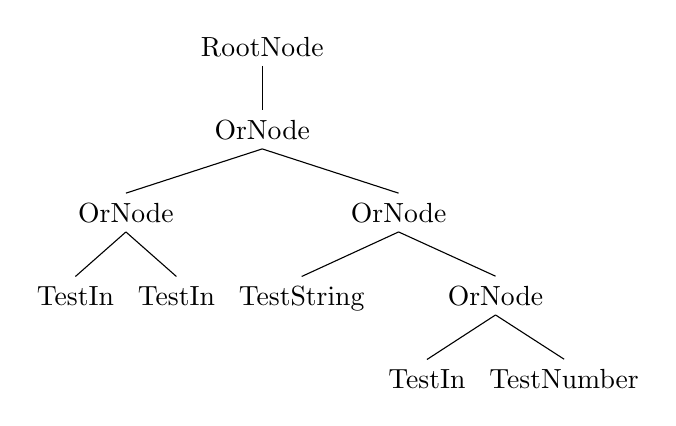
\begin{tikzpicture}
\Tree [.RootNode
	[.OrNode
		[.OrNode
			TestIn
			TestIn
		]
		[.OrNode
			TestString
			[.OrNode
				TestIn
				TestNumber
			]
		]
	]
]
\end{tikzpicture}}
	\caption{Árbore de sintaxe de exemplo}
	\label{fig:arborenodos}
\end{figure}

Decidiuse usar un método recursivo, e non iterativo, por que resultaba máis sinxelo implementalo e non se considera que as posibles peticións que se fixeran poidan sobrepasar o límite da pila de chamadas. De todos xeitos, o uso dos operadores lóxicos de Java (\texttt{\&\&} e \texttt{||}) con cortocircuíto reducen tamén o número de operacións a realizar.

Para implementar a paxinación úsase unha caché LRU, que usando coma índice do mapa a petición devolve unha listaxe de obxectos comprobados para esa petición. Existe unha caché para cada tipo de obxecto.

As propiedades dispoñibles son:

\begin{itemize}
	\item template.name
	\item template.description
	\item template.field.name
	\item template.field.type
	\item component.name
	\item component.description
	\item component.field.name
	\item component.field.type
	\item component.field.value
	\item user.name
	\item user.email
	\item user.role
\end{itemize}

Comparar un valor dun campo só devolverá os compoñentes con campos do tipo axeitado (\texttt{TEXT}, \texttt{DATETIME} para as cadeas; \texttt{NUMBER}, \texttt{LINK} e \texttt{DATETIME} para os números). Para comparar con propiedades que conteñan enumeracións, deberá usarse o nome orixinal da enumeración, non o que poida amosar a interface web.
 %% https://tex.stackexchange.com/a/587535
\newcommand{\newthreadShift}[4][gray!30]{
  \newinst[#4]{#2}{#3}
  \stepcounter{threadnum}
  \node[below of=inst\theinstnum,node distance=0.8cm] (thread\thethreadnum) {};
  \tikzstyle{threadcolor\thethreadnum}=[fill=#1]
  \tikzstyle{instcolor#2}=[fill=#1]
}

\chapter{Seguridade: Autenticación e autorización}
\label{chap:seguridade}

Dentro da aplicación existen dous ámbitos de seguridade: o presente na parte servidor, e o presente na parte do cliente.

\section{Servidor}

Dentro do servidor, xúntanse autenticación e autorización. No servidor úsase Jakarta para xestionar a autorización, dentro da clase propia \texttt{AuthenticationManager}, etiquetada axeitadamente para que se poida incluír na cadea de filtros sen precisar de configuración. Esta clase implanta a interface \texttt{ContainerRequestFilter}, de xeito que Jakarta inclúea coma filtro cando recibe unha petición.\cite{jakartafilter}

É aquí onde se decide se se permite o acceso, e se se continúa cos filtros ate chegar aos controladores, que son os que procesan as peticións REST. O algoritmo aquí usa, para decidir, o rol do usuario, a ruta e o método a acceder. Máis abaixo explicarase con detalle o proceso.

Sen unha identificación válida, só se permite o acceso á ruta \texttt{/users/login} por POST, por precisarse para iniciar sesión.

Os usuarios con rol ADMINISTRATOR teñen acceso ilimitado ao sistema, mentres que os usuarios co rol NORMAL\_USER teñen vedada a modificación de todo excepto compoñentes, polo tanto só poden acceder a:

\begin{description}
    \item[POST]
        \begin{itemize}
            \item \texttt{/users/(id)/logout}: Esta ruta precísase para pechar a sesión.
            \item \texttt{/components/*}
        \end{itemize}
    \item[GET]
        \begin{itemize}
            \item \texttt{/users/*}
            \item \texttt{/templates/*}
        \end{itemize}
\end{description}

Como a xestión de usuarios é dominio exclusivo dos administradores, tampouco se lle permite a un técnico modificar o seu propio usuario. Enténdese que a creación do usuario responde a políticas empresariais, e probablemente en versións futuras dependa de sistemas de usuarios.

O fluxo de inicio de sesión é o amosado no diagrama da figura \ref{fig:loginsrv}\footnote{O que hai entre parénteses é o corpo da petición}:

\begin{figure}[H]
    \centering
\begin{sequencediagram}
    \newthread{A}{Cliente}{}
    \newthreadShift{B}{Servidor}{5}
    \newthreadShift{C}{Base de datos}{3}
    \postlevel 
    \begin{call}{A}{\shortstack{POST /users/login?user=usuario \\ (contrasinal)}}{B}{200 OK (token)}
        \begin{call}{B}{getUserByName}{C}{User}
        \end{call}
    \end{call}
\end{sequencediagram}
    \caption{Fluxo de inicio de sesión no servidor}
    \label{fig:loginsrv}
\end{figure}

Tras recibir o usuario, se o contrasinal (enviado en texto plano e cifrado no servidor) coincide co gardado na base de datos, o servidor xera unha \Gls{testemuna} aleatoria\footnote{Xerada a partir da clase \texttt{Random} de Java} que devolve ao cliente. Se o contrasinal non coincide, ou non se atopou o usuario indicado, devólvese un código 404 e a mensaxe «\textit{User not found}».

Despois diso todas as peticións enviarán a testemuña nunha cabeceira, chamada \texttt{X-API-KEY}. Esta cabeceira será comprobada, tal como se indicou arriba, polo filtro \texttt{AuthenticationManager}, que comprobará a súa validez e os permisos asignados ao usuario que a creou. Isto pode verse no diagrama da figura \ref{fig:authsrv}

\begin{figure}[H]
    \centering
    \begin{sequencediagram}
    \newthread{A}{Cliente}{}
    \newthreadShift{B}{Servidor}{5}
    \newthreadShift{C}{Base de datos}{3}
    \postlevel 
    \begin{call}{A}{
        \shortstack{
            Petición \\
            X-API-HEADER: token}
    }{B}{Resposta}
        \begin{call}{B}{getUserByToken}{C}{User}
        \end{call}
    \end{call}
\end{sequencediagram}
    \caption{Fluxo de acceso á API}
    \label{fig:authsrv}
\end{figure}

Se o filtro non atopa a testemuña na base de datos, devolverá unha mensaxe \texttt{404 Not Found}, mentres que se atopa a testemuña, pero o usuario asociado non ten o rol axeitado, devolverá unha mensaxe \texttt{403 Forbidden}.\footnote{Tal coma se indica na sección 6.5.3 do RFC 7321\cite{rfc7231}}

Por último, só queda explicar a ruta \texttt{/users/(id)/logout}. Esta ruta, que precisa dunha testemuña válida para acceder, o único que fai é eliminar a testemuña que se lle pase polo corpo da mensaxe. Se non existe a testemuña baixo este usuario, devolve unha mensaxe \texttt{404 Not Found}. Polo tanto, o fluxo completo quedaría tal coma se indica no diagrama da figura \ref{fig:totalsrv}

\begin{figure}[H]
    \centering
\begin{sequencediagram}
    \newthread{A}{Cliente}{}
    \newthreadShift{B}{Servidor}{5}
    \postlevel
    \begin{call}{A}{Iniciar sesión (Ver figura \ref{fig:loginsrv})
    }{B}{Testemuña}
    \setthreadbias{center}
    \end{call}
    \postlevel
    \begin{sdblock}{Bucle}{}
        \begin{call}{A}{Petición figura (Ver \ref{fig:authsrv})
        }{B}{Resposta}
        \end{call}
    \end{sdblock}
    \postlevel
    \postlevel
    \begin{call}{A}{
        \shortstack{
            POST  /users/(id)/logout \\
            X-API-HEADER: token \\
            (token)}
    }{B}{204 No Content}
    \end{call}
\end{sequencediagram}
    \caption{Proceso completo de acceso á API}
    \label{fig:totalsrv}
\end{figure}

\section{Cliente}

Na parte do cliente ambas, tanto a autenticación como a autorización, están xestiónaas Spring Security. Isto funciona mediante a implementación local de varias clases, que Spring encárgase de integrar no sistema.

\newpage

De xeito semellante ao servidor, o sistema baséase nunha serie de filtros\cite{springsecarch} que deciden se permiten ou non o acceso. Para un usuario externo, o proceso sería o seguinte:

\begin{enumerate}
    \item O usuario intenta acceder á ruta /
    \item Spring invoca unha instancia da interface \texttt{Authorization\allowbreak{}Manager}, pasándolle coma obxecto un \texttt{Anonymous\allowbreak{}Authentication\allowbreak{}Token}
    \item Se o \texttt{Authorization\allowbreak{}Manager} denega acceso, Spring redirixe ao usuario a unha ruta indicada para que inicie sesión, neste caso \texttt{/login}
    \item Tras introducir as credenciais, Spring invoca unha instancia da clase \texttt{Authentication\allowbreak{}Provider}, pasándolle unha clase \texttt{Username\allowbreak{}Password\allowbreak{}Authentication\allowbreak{}Token}. Esta clase decide se as credenciais son correctas, e nese caso devolve unha autenticación.
    \item O usuario rediríxese á páxina de inicio
\end{enumerate}

Tras isto, gárdase a testemuña dentro do almacenamento da sesión, e recupérase para facer peticións. Cada vez que o usuario acceda a unha nova ruta, Spring chamará a \texttt{Authorization\allowbreak{}Manager} antes de permitilo.

No caso desta aplicación, todo isto configúrase na clase \texttt{pleste.\allowbreak{}client.\allowbreak{}Security\allowbreak{}Config}. Nesta clase defínese un método

\begin{lstlisting}[language=Java]
@Bean
public SecurityFilterChain filterChain(HttpSecurity http,
    AuthorizationManager<RequestAuthorizationContext> authorizationManager)
    throws Exception {
\end{lstlisting}

que, usando unha DSL formada mediante métodos da clase \texttt{HttpSecurity} e usando o patrón construtor, permiten segregar os métodos de autorización segundo a ruta á que se acceda:

\begin{lstlisting}[language=Java]
return http.csrf(AbstractHttpConfigurer::disable)
    .authorizeHttpRequests(
        authorizationManagerRequestMatcherRegistry ->
            authorizationManagerRequestMatcherRegistry
                .requestMatchers("/login*").anonymous())
\end{lstlisting}

Todos os métodos de autorizar peticións seguen o mesmo formato: a ruta a comprobar dentro do lambda, seguido do tipo de acceso permitido. Neste caso, o acceso anónimo permite que só os usuarios que inda non iniciaron sesión poidan acceder ao formulario de inicio de sesión.

\begin{lstlisting}[language=Java]
    .authorizeHttpRequests(
        authorizationManagerRequestMatcherRegistry ->
            authorizationManagerRequestMatcherRegistry
                .requestMatchers("/favicon*", "/logout*", "/css/*",
                    "/js/*", "/error*").permitAll())
\end{lstlisting}

Aquí contrólanse certas rutas relacionadas con recursos (\textit{favicon}, CSS e JS) e cousas técnicas (\texttt{/logout} e \texttt{/error}). En todos estes casos permítese acceso indiscriminado, sen importar se se iniciou sesión ou non.

\begin{lstlisting}[language=Java]
    .authorizeHttpRequests(
        authorizationManagerRequestMatcherRegistry ->
            authorizationManagerRequestMatcherRegistry
                .requestMatchers("/**").access(authorizationManager))
\end{lstlisting}

Esta é a regra por omisión. Para o resto de rutas, precísase iniciar sesión, usando a clase authorizationManager (inxectada por Spring mediante parámetro).

\begin{lstlisting}[language=Java]
    .formLogin(httpSecurityFormLoginConfigurer ->
        httpSecurityFormLoginConfigurer
            .loginPage("/login")
            .successForwardUrl("/")
            .failureForwardUrl("/login?error=true"))
\end{lstlisting}

Nesta parte indícaselle a Spring Security como funciona o formulario de inicio de sesión personalizado. Indícase a ruta a acceder en caso de non iniciar sesión (\texttt{/login}), a onde redirixir en caso de que o inicio de sesión funcione (\texttt{/}) e en caso de que non (\texttt{/login?error=true}).

\begin{lstlisting}[language=Java]
    .logout(
        httpSecurityLogoutConfigurer -> httpSecurityLogoutConfigurer
            .addLogoutHandler(new LocalLogoutHandler(defaultApi))).build();
\end{lstlisting}

Para rematar, tamén configúrase o peche de sesión. Neste caso engádese a clase que Spring chamará en caso de intentar acceder a \texttt{/logout}.

Unha vez configurado todo, queda implementar as clases precisas para que a autenticación e autorización fágase mediante peticións REST ao servidor. Amósase de exemplo como sería o fluxo típico dun usuario accedendo á aplicación.

\newpage

Para iniciar sesión o fluxo sería o amosado no diagrama da figura \ref{fig:logincliente}:

\begin{figure}[H]
    \centering
\begin{sequencediagram}
    \newthread{U}{Usuario}{}
    \newthreadShift{C}{Cliente}{5}
    \newthreadShift{S}{Servidor}{5}
    \begin{call}{U}{Acceder a /}{C}{Redirixe a /login}
        \begin{call}{C}{Póde acceder a /?}{C}{Non}
        \end{call}
    \end{call}
    \begin{call}{U}{Envía formulario de /login}{C}{Redirixe a /}
        \begin{call}{C}{POST /users/login (ver figura \ref{fig:loginsrv})}{S}{200 OK (token)}            
        \end{call}
    \end{call}
\end{sequencediagram}
    \caption{Acceso á aplicación por parte dun usuario anónimo}
    \label{fig:logincliente}
\end{figure}

Aquí encárgase de iniciar sesión a clase \texttt{Local\allowbreak{}Authentication\allowbreak{}Provider}, que implementa a interface \texttt{Authentication\allowbreak{}Provider}. Esta clase é a encargada de, tras recibir o usuario e contrasinal dende o formulario de inicio de sesión, comunicarse co servidor e validar os datos do usuario. Tras facer isto, garda no almacenamento da sesión o nome de usuario, id e testemuña para uso futuro. Para gardar o resultado da autenticación creouse unha clase \texttt{Local\allowbreak{}Authentication}, que implementa a interface \texttt{Authentication} esta clase só é un almacén de datos compatible cos subsistemas do módulo de \textit{Spring Security}.

Unha vez iniciada sesión, calquera ruta na que intente acceder o cliente seguirá o proceso amosado no diagrama da figura \ref{fig:normalcliente}:

\begin{figure}[H]
    \centering
\begin{sequencediagram}
    \newthread{U}{Usuario}{}
    \newthreadShift{C}{Cliente}{5}
    \newthreadShift{S}{Servidor}{5}
    \begin{call}{U}{Acceso a unha ruta}{C}{Devolve  vista}
        \begin{call}{C}{LocalAuthorizationManager}{C}{AuthorizationDecision(true)}
            \begin{call}{C}{GET /users/(id)/role}{S}{200 OK (TypeRole)}
            \end{call}
        \end{call}
    \end{call}
\end{sequencediagram}
    \caption{Uso típico no cliente}
    \label{fig:normalcliente}
\end{figure}

\newpage

Neste proceso, Spring Security chama á clase \texttt{Local\allowbreak{}Authorization\allowbreak{}Manager}, que implementa a interface \texttt{Authorization\allowbreak{}Manager}. Esta clase encárgase de buscar o rol do usuario actual, usando para iso o usuario que Spring lle pasa mediante un parámetro \texttt{Local\allowbreak{}Authentication}, e comprobando que o dito rol pode acceder á ruta indicada. Unha vez confirmado isto, devolve unha instancia da clase \texttt{Authorization\allowbreak{}Decision(true)} afirmando que o usuario pode acceder ao recurso. Feito isto, Spring continúa procesando a petición e devolve a vista axeitada (para máis información, consulte o capítulo \ref{chap:gui}).

Para rematar, amósase o fluxo de peche de sesión no diagrama da figura \ref{fig:logoutcliente}:

\begin{figure}[H]
    \centering
\begin{sequencediagram}
    \newthread{U}{Usuario}{}
    \newthreadShift{C}{Cliente}{5}
    \newthreadShift{S}{Servidor}{5}
    \begin{call}{U}{Preme en «Pechar Sesión»}{C}{Redirixe a /login}
        \begin{call}{C}{POST /users/(id)/logout (token)}{S}{204 No Content)}            
        \end{call}
    \end{call}
\end{sequencediagram}
    \caption{Pechar sesión}
    \label{fig:logoutcliente}
\end{figure}

Neste caso tamén intervén unha clase propia, \texttt{Local\allowbreak{}Logout\allowbreak{}Handler}, que implementa a interface \texttt{Logout\allowbreak{}Handler}. Esta clase o único que fai é facer unha petición ao servidor para que elimine a testemuña (véxase o final da figura \ref{fig:totalsrv}), e limpa o almacenamento da sesión. Sexa como for, Spring Security da por rematada a sesión e volve tratar o usuario coma anónimo.

Todo isto xunto da, coma fluxo final, o amosado no diagrama da figura \ref{fig:totalcliente}:

\begin{figure}[htbp]
    \centering
\begin{sequencediagram}
    \newthread{U}{Usuario}{}
    \newthreadShift{C}{Cliente}{5}
    \newthreadShift{S}{Servidor}{5}
    \begin{call}{U}{Acceder a /}{C}{Redirixe a /login}
        \begin{call}{C}{Póde acceder a /?}{C}{Non}
        \end{call}
    \end{call}
    \begin{call}{U}{Envía formulario de /login}{C}{Redirixe a /}
        \begin{call}{C}{POST /users/login}{S}{200 OK (token)}            
        \end{call}
    \end{call}
    \begin{sdblock}{Bucle}{Todos os accesos seguen este proceso}
        \begin{call}{U}{Acceso a unha ruta}{C}{Devolve  vista}
            \begin{call}{C}{LocalAuthorizationManager}{C}{AuthorizationDecision(true)}
                \begin{call}{C}{GET /users/(id)/role}{S}{200 OK (TypeRole)}
                \end{call}
            \end{call}
        \end{call}
    \end{sdblock}
    \begin{call}{U}{Preme en «Pechar Sesión»}{C}{Redirixe a /login}
        \begin{call}{C}{POST /users/(id)/logout (token)}{S}{204 No Content)}            
        \end{call}
    \end{call}
\end{sequencediagram}
    \caption{Uso típico no cliente}
    \label{fig:totalcliente}
\end{figure}
 \chapter{Conclusións}
\label{chap:conclusions}

Como conclusión do proxecto, o traballo acadado preséntase cun balance positivo, non só polo programa creado e xa descrito nesta memoria, senón que tamén por todo o proceso de aprendizaxe realizado ante tantas ferramentas e tecnoloxías practicamente novas. Inda que a base bebe moito do aprendido durante a carreira, especialmente da materia de \textit{Integración de Aplicacións}, a experiencia de montar o proxecto dende cero e engadindo novas tecnoloxías resultou didáctica, tanto nos acertos coma nos fallos no deseño da aplicación.

Por desgraza, e a pesar da axuda prestada polos directores do proxecto, esta plataforma inda precisa probarse nun ambiente real, tras o cal seguramente se precisen facer máis melloras para adaptalo a unha carga de traballo real. Entre outras, seguramente se precisará dunha integración cun sistema de identificación e autenticación externo. Porén, por mor da falta de tempo decidiuse reducir o alcance do proxecto ao actual.

Por sorte, o deseño empregado na construción da plataforma permite unha adaptación sinxela a calquera engadido que se lle queira realizar en datas futuras.

\section{Futuras melloras}

Sexa como for, existen varias melloras posibles á aplicación, que por falta de tempo e dificultade, ou outros motivos, non se puideron engadir.

A posibilidade máis útil é a integración con outras ferramentas xa existentes. A API actual presenta unha interface completa dabondo para que outras aplicacións poidan xestionar o contido da base de datos, pero esta integración só e unidireccional. Actualmente non existe ningún xeito de executar accións automáticas, nin realizar interaccións activas con outras aplicacións. Probablemente isto precisará engadir un novo tipo de entidade á aplicación, que usando algunha linguaxe dinámica (Lisp ou Lua, por exemplo) permita definir condicións de activación e accións a executar.

\newpage

Unha característica que quedou fora da aplicación é un rexistro. Facer un sistema de rexistro útil precisaría de rexistrar todas as actividades que realiza a aplicación, vinculándoas a un usuario e obxecto precisos.

Xunto cunha futura integración cun sistema de autenticación externo, poderíase engadir un sistema de permisos máis detallado e configurable.

Unha característica menor, pero que precisaríase para unha futura expansión da aplicación, é a localización. Actualmente a aplicación inserta directamente cadeas de texto dentro das páxinas da aplicación e das mensaxes dos fallos. Centralizar todo isto axudaría á tradución e arranxar erratas.

 %%%%%%%%%%%%%%%%%%%%%%%%%%%%%%%%%%%%%%%%
 % Apéndices, glosarios e bibliografía  %
 %%%%%%%%%%%%%%%%%%%%%%%%%%%%%%%%%%%%%%%%

 \appendix
 \appendixpage
 \chapter{Material adicional}
\label{chap:adicional}

Pódese acceder ao código desta aplicación dende a ruta \url{https://github.com/Parodper/tfg_plataforma_xestion_tecnica/}
%\include{anexos/...}

 \printglossary[type=\acronymtype,title=\nomeglosarioacronimos]
 \printglossary[title=\nomeglosariotermos]

 \bibliographystyle{IEEEtranN}
 \bibliography{\bibconfig,bibliografia/bibliografia}
 \clearpage
 
\end{document}

%%%%%%%%%%%%%%%%%%%%%%%%%%%%%%%%%%%%%%%%%%%%%%%%%%%%%%%%%%%%%%%%%%%%%%%%%%%%%%%%
